\documentclass[11pt,a4paper]{article}

\usepackage[margin=1in]{geometry}
\usepackage[hidelinks]{hyperref}
\usepackage{enumitem}
\usepackage{graphicx}
\usepackage{xcolor}
\usepackage{titling}

% TikZ packages for workflow diagrams
\usepackage{tikz}
\usetikzlibrary{positioning,arrows.meta,shapes.geometric,fit}

% Improve line breaking and reduce overfull hbox warnings
\setlength{\emergencystretch}{3em}
\sloppy

% -----------------------------------------------------
% bvraghav-tiet-ucs503p-article.sty
% -----------------------------------------------------

% Variable: Lab Instructor
\makeatletter

\newcommand{\BvrSetLabInstructor}[1]{%
\gdef\Bvr@LabInstructor{#1}}

% Default
\newcommand{\Bvr@LabInstructor}{Dr. Raghav B. Venkataramaiyer}

% Public accessor
\newcommand{\BvrLabInstructorValue}{\Bvr@LabInstructor}

\makeatother

% -----------------------------------------------------
% Title formatting
% -----------------------------------------------------

\pretitle{\begin{center}\bfseries\Large}

\makeatletter

\newcommand{\BvrSubtitle}[1]{%
\posttitle{%
\par\end{center}
\begin{center}\large#1\end{center}
\vskip 0.5em}%
}

\makeatother

% -----------------------------------------------------
% Hints in section titles (disabled)
% -----------------------------------------------------

\newcommand{\BvrHint}[1]{}

% -----------------------------------------------------
% Title
% -----------------------------------------------------

\title{AI-Powered Log Analysis \& Incident Triage System}

\BvrSetLabInstructor{Dr. Jeelani Asif}

\BvrSubtitle{%
Project Proposal for UCS503P \\
Submitted to: \BvrLabInstructorValue \\ \bfseries
Thapar Institute of Engineering and Technology%
}

\author{
Arnav Singh, CSED%
\thanks{Roll No: \texttt{1024160011}, %
Email: \texttt{asingh30\_be24@thapar.edu}}
\and
Siddharth Chandra, CSED%
\thanks{Roll No: \texttt{1024160017}, %
Email: \texttt{schadra\_be24@thapar.edu}}
}

\date{August 12, 2026}

% =====================================================
% DOCUMENT
% =====================================================

\begin{document}

\maketitle

% -----------------------------------------------------
% 1. Higher-order goal
% -----------------------------------------------------

\section{Higher-order goal}

This project aims to improve modern DevOps and software system reliability by drastically reducing the time and manual effort required to diagnose application failures. While system monitoring spans vast cloud infrastructures, the immediate engineering objective is to translate automated log parsing and LLM-driven root cause analysis (RCA) into a measurable, deployable, and developer-centric software platform.

% -----------------------------------------------------
% 2. Time-to-value
% -----------------------------------------------------

\section{Time-to-value}

We will deliver meaningful increments quickly by prototyping the core log ingestion and triage workflow and validating it within a 10-week Agile development window across 2-week Sprint iterations.

We will prioritize fast feedback over perfection by utilizing bi-weekly Sprint reviews and automated CI/CD pipelines early to eliminate release friction. Success is defined by what can be delivered and measured in the initial iteration, then iteratively expanded based on system telemetry and user testing.

% -----------------------------------------------------
% 3. Problem Statement
% -----------------------------------------------------

\section{Problem Statement}

Software engineering and Site Reliability Engineering (SRE) teams managing distributed microservices face severe delays and operational fatigue during system outages. Common pain points include:

\begin{itemize}[leftmargin=0.7cm]

\item \textbf{Fragmentation:} Log data is scattered across multiple services, containers, and isolated text files, causing lost context during incidents.

\item \textbf{Low Transparency \& High Noise:} Standard logging tools display thousands of cryptic, raw stack traces without explaining the actual failure trigger or severity.

\item \textbf{Slow Incident Coordination:} On-call engineers lack a unified, automated triage workflow, spending up to 70\% of incident response time manually tracing root causes.

\item \textbf{Alert Fatigue:} High volume and duplicate error streams flood alerting channels, leading to missed critical failures and extended Mean Time to Resolution (MTTR).

\end{itemize}

\textbf{Why this matters now:} In modern high-availability applications, even minor downtime incidents incur significant financial losses; reducing diagnosis time directly protects service reliability.

% -----------------------------------------------------
% 4. Proposed Solution
% -----------------------------------------------------

\section{Proposed Solution}

\subsection{Overview}

Build a web-based \textbf{AI-Powered Log Analysis \& Incident Triage System} comprising the following components:

\begin{itemize}[leftmargin=0.7cm]

\item \textbf{Log Ingestion Engine:} High-throughput API pipeline to ingest, parse, and index structured and unstructured log batches in real time.

\item \textbf{Automated AI Triage \& RCA:} LLM-driven error classification, stack trace translation, and root-cause analysis (RCA) generation.

\item \textbf{Incident Management Workflow:} Real-time stream filtering, error velocity tracking, and incident status updates (\texttt{Open} $\rightarrow$ \texttt{Investigating} $\rightarrow$ \texttt{Resolved}).

\item \textbf{Real-Time Dashboard \& Alerts:} WebSocket-powered dashboard featuring error rate charts and automated webhook alerts (Slack/Discord).

\end{itemize}

% -----------------------------------------------------
% Core Workflow
% -----------------------------------------------------

\subsection{Core Workflow}

\begin{enumerate}[leftmargin=0.7cm]

\item Microservices emit log payloads to the central ingestion REST endpoint.

\item The ingestion pipeline parses incoming stack traces, performs caching/deduplication in Redis, and indexes entries in PostgreSQL/Elasticsearch.

\item For anomalous error spikes or critical exceptions, the system triggers the LLM inference engine to synthesize a plain-language RCA report and suggested remediation steps.

\item Engineers review the live dashboard, receive automated notifications, and update incident statuses upon resolution.

\end{enumerate}

% -----------------------------------------------------
% Figure 1: End-to-End Core Workflow
% -----------------------------------------------------

\begin{figure}[htbp]
\centering

\resizebox{\textwidth}{!}{%
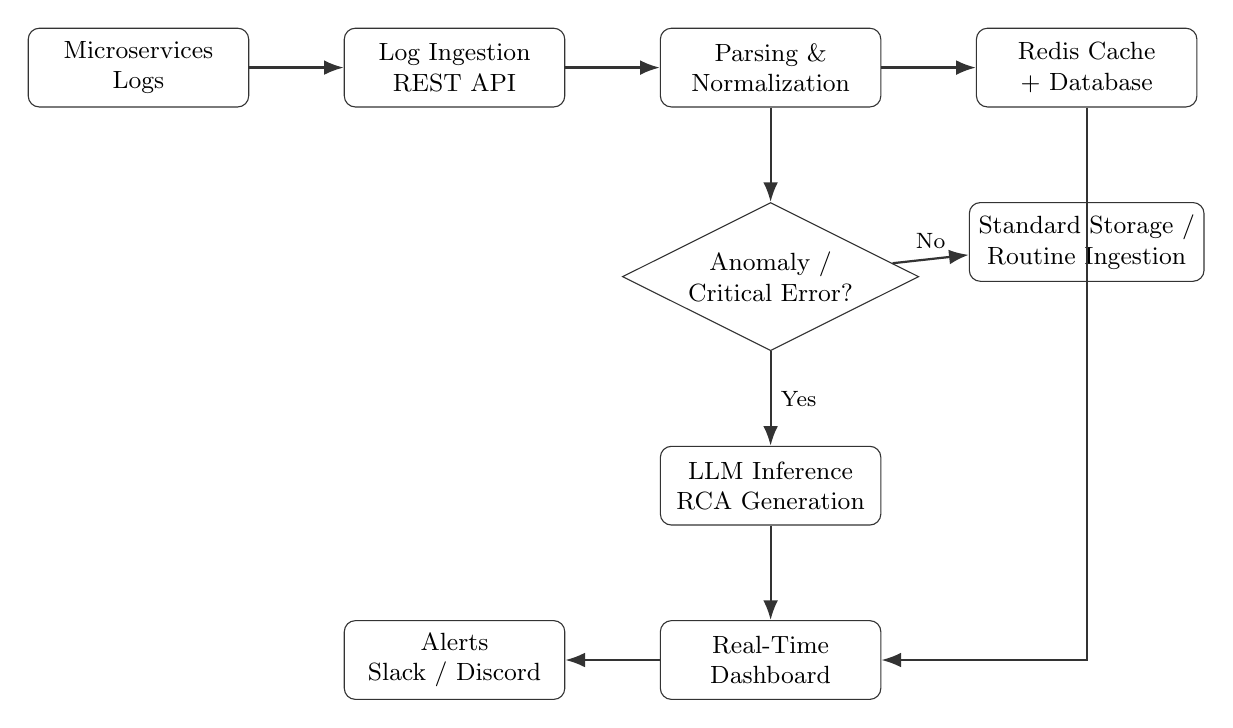
\begin{tikzpicture}[
    node distance=1.2cm and 1.2cm,
    box/.style={
        rectangle,
        rounded corners=4pt,
        draw=black!80,
        fill=white,
        align=center,
        minimum width=2.8cm,
        minimum height=1.0cm,
        font=\small
    },
    decision/.style={
        diamond,
        draw=black!80,
        fill=white,
        align=center,
        aspect=2,
        inner sep=2pt,
        font=\small
    },
    arrow/.style={
        -{Latex[length=2.5mm]},
        thick,
        draw=black!80
    }
]

% Top Row: Ingestion Pipeline
\node[box] (logs) {Microservices\\Logs};
\node[box, right=of logs] (ingestion) {Log Ingestion\\REST API};
\node[box, right=of ingestion] (processing) {Parsing \&\\Normalization};
\node[box, right=of processing] (storage) {Redis Cache\\+\ Database};

% Middle Row: Anomaly Decision & Processing Branches
\node[decision, below=1.2cm of processing] (anomaly) {Anomaly /\\Critical Error?};
\node[box, below=1.2cm of storage] (engineer) {Standard Storage /\\Routine Ingestion};
\node[box, below=1.2cm of anomaly] (llm) {LLM Inference\\RCA Generation};

% Bottom Row: Dashboard & Alerts
\node[box, below=1.2cm of llm] (dashboard) {Real-Time\\Dashboard};
\node[box, left=of dashboard] (alerts) {Alerts\\Slack / Discord};

% Connections
\draw[arrow] (logs) -- (ingestion);
\draw[arrow] (ingestion) -- (processing);
\draw[arrow] (processing) -- (storage);
\draw[arrow] (processing) -- (anomaly);

\draw[arrow] (anomaly) -- node[above, font=\footnotesize] {No} (engineer);
\draw[arrow] (anomaly) -- node[right, font=\footnotesize] {Yes} (llm);

\draw[arrow] (llm) -- (dashboard);
\draw[arrow] (dashboard) -- (alerts);
\draw[arrow] (storage) |- (dashboard);

\end{tikzpicture}%
}

\caption{End-to-End Log Analysis and Incident Triage Workflow}
\label{fig:core-workflow}

\end{figure}

% -----------------------------------------------------
% Operational Constraints
% -----------------------------------------------------

\subsection{Operational Constraints}

\begin{itemize}[leftmargin=0.7cm]

\item Keep the dashboard UI responsive and intuitive on standard web browsers.

\item Focus heavily on robust workflow engineering, stream processing, caching, and system correctness rather than training custom foundational LLMs.

\item Design for containerized deployment using standard platform hosting and managed databases.

\end{itemize}

% -----------------------------------------------------
% 5. Solution Approach
% -----------------------------------------------------

\section{Solution Approach}

\subsection{AI \& Deduplication Assistance}

Duplicate log handling and root cause analysis will rely on heuristic and inference-driven strategies:

\begin{itemize}[leftmargin=0.7cm]

\item Normalize incoming log messages by stripping dynamic parameters (e.g., timestamps, memory addresses).

\item Use Redis caching to store generated AI analyses for identical error signatures, preventing redundant API calls during error storms.

\item Present LLM-generated RCA summaries and suggested fixes directly to engineers to assist human decision-making.

\end{itemize}

% -----------------------------------------------------
% System Architecture
% -----------------------------------------------------

\subsection{System Architecture}

A modern 3-tier decoupling model:

\begin{itemize}[leftmargin=0.7cm]

\item \textbf{Frontend:} Responsive React dashboard for real-time log tailing, error velocity visualizer, and incident inspection.

\item \textbf{Backend API:} FastAPI (Python) web service handling REST ingestion, WebSocket connections, LLM prompt orchestration, and alert triggers.

\item \textbf{Data \& Cache Layer:} PostgreSQL/Elasticsearch for persistent query indexing, and Redis for rate-limiting and response caching.

\end{itemize}

% -----------------------------------------------------
% Figure 2: System Architecture
% -----------------------------------------------------

\begin{figure}[htbp]
\centering

\resizebox{\textwidth}{!}{%
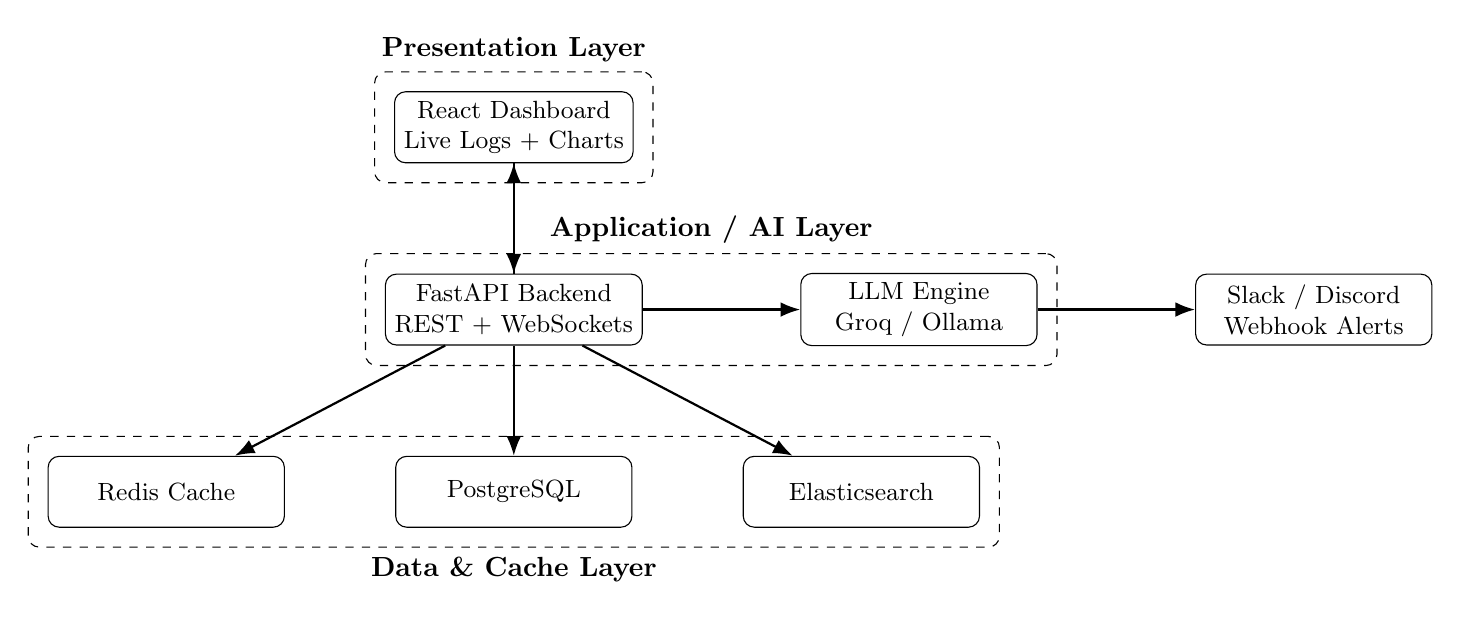
\begin{tikzpicture}[
    node distance=1.4cm and 1.3cm,
    box/.style={
        rectangle,
        rounded corners,
        draw,
        align=center,
        minimum width=3.0cm,
        minimum height=0.9cm,
        font=\small
    },
    arrow/.style={
        -{Latex[length=2.5mm]},
        thick
    }
]

% Frontend
\node[box] (react)
{React Dashboard\\
Live Logs + Charts};

% Backend
\node[box, below=1.4cm of react] (fastapi)
{FastAPI Backend\\
REST + WebSockets};

% AI
\node[box, right=2.0cm of fastapi] (llm)
{LLM Engine\\
Groq / Ollama};

% Data layer
\node[box, below=1.4cm of fastapi] (postgres)
{PostgreSQL};

\node[box, right=1.4cm of postgres] (elastic)
{Elasticsearch};

\node[box, left=1.4cm of postgres] (redis)
{Redis Cache};

% Alerts
\node[box, right=2.0cm of llm] (alerts)
{Slack / Discord\\
Webhook Alerts};

% Connections
\draw[arrow] (react) -- (fastapi);

\draw[arrow] (fastapi) -- (llm);

\draw[arrow] (fastapi) -- (postgres);

\draw[arrow] (fastapi) -- (elastic);

\draw[arrow] (fastapi) -- (redis);

\draw[arrow] (llm) -- (alerts);

\draw[arrow] (fastapi) -- (react);

% Layer boxes
\node[
    rectangle,
    rounded corners,
    draw,
    dashed,
    inner sep=7pt,
    fit=(react),
    label=above:{\textbf{Presentation Layer}}
] {};

\node[
    rectangle,
    rounded corners,
    draw,
    dashed,
    inner sep=7pt,
    fit=(fastapi)(llm),
    label=above:{\textbf{Application / AI Layer}}
] {};

\node[
    rectangle,
    rounded corners,
    draw,
    dashed,
    inner sep=7pt,
    fit=(redis)(postgres)(elastic),
    label=below:{\textbf{Data \& Cache Layer}}
] {};

\end{tikzpicture}%
}

\caption{Three-Tier System Architecture}
\label{fig:architecture}

\end{figure}

% -----------------------------------------------------
% CI/CD
% -----------------------------------------------------

\subsection{CI/CD and Fast Delivery Enabler}

CI/CD pipelines will be configured to:

\begin{itemize}[leftmargin=0.7cm]

\item Run automated linting, unit tests, and integration tests on every commit.

\item Produce containerized Docker artifacts for repeatable staging and production deployments.

\item Enable seamless, incremental releases across each Agile Sprint.

\end{itemize}

% -----------------------------------------------------
% Figure 3: CI/CD Workflow
% -----------------------------------------------------

\begin{figure}[htbp]
\centering

\resizebox{\textwidth}{!}{%
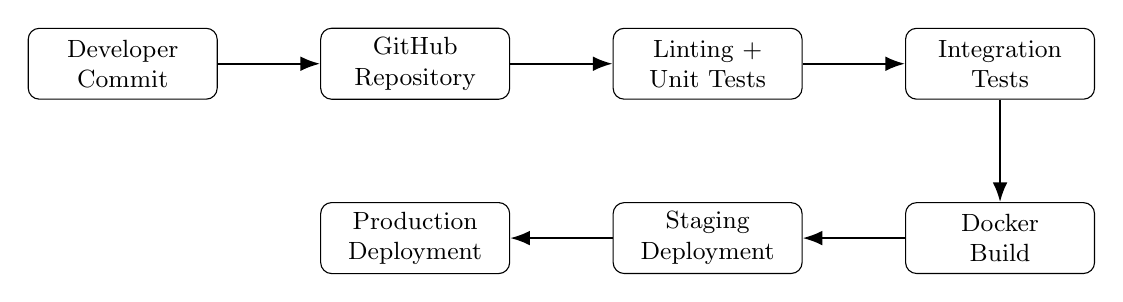
\begin{tikzpicture}[
    node distance=1.3cm,
    box/.style={
        rectangle,
        rounded corners,
        draw,
        align=center,
        minimum width=2.4cm,
        minimum height=0.9cm,
        font=\small
    },
    arrow/.style={
        -{Latex[length=2.5mm]},
        thick
    }
]

\node[box] (commit)
{Developer\\Commit};

\node[box, right=of commit] (github)
{GitHub\\Repository};

\node[box, right=of github] (tests)
{Linting +\\Unit Tests};

\node[box, right=of tests] (integration)
{Integration\\Tests};

\node[box, below=1.3cm of integration] (docker)
{Docker\\Build};

\node[box, left=of docker] (staging)
{Staging\\Deployment};

\node[box, left=of staging] (production)
{Production\\Deployment};

\draw[arrow] (commit) -- (github);
\draw[arrow] (github) -- (tests);
\draw[arrow] (tests) -- (integration);
\draw[arrow] (integration) -- (docker);
\draw[arrow] (docker) -- (staging);
\draw[arrow] (staging) -- (production);

\end{tikzpicture}%
}

\caption{Automated CI/CD Pipeline}
\label{fig:cicd}

\end{figure}

% -----------------------------------------------------
% 6. Evaluation Criteria
% -----------------------------------------------------

\section{Evaluation Criteria}

\subsection{Primary Evaluation Metric}

\textbf{Mean Time to Diagnosis (MTTD):} The duration between a critical log error entering the system and an automated RCA report being generated and displayed.

\begin{itemize}[leftmargin=0.7cm]

\item \textit{Target:} Median MTTD $< 5$ seconds during stress testing.

\item \textit{Attribution:} Measured via backend processing timestamps (ingestion log time vs. LLM output completion time).

\end{itemize}

\subsection{Secondary Evaluation Metrics}

\begin{itemize}[leftmargin=0.7cm]

\item \textbf{Log Ingestion Throughput:} Sustained logs processed per second without dropped connection payloads.

\item \textbf{Cache Hit Rate:} Percentage of duplicate error traces served via Redis without hitting external LLM endpoints.

\item \textbf{System Uptime \& Reliability:} Availability of dashboard and API ingestion endpoints during test runs ($>99\%$ operational target).

\end{itemize}

% -----------------------------------------------------
% 7. Scalability \& Agile Delivery Roadmap
% -----------------------------------------------------

\section{Scalability \& Agile Delivery Roadmap}

\subsection{Scalability Considerations}

\begin{itemize}[leftmargin=0.7cm]

\item \textbf{Theoretically:} Decoupled architecture using asynchronous event loops in FastAPI, stateless REST routes, and indexed database lookups to handle heavy log traffic spikes.

\item \textbf{Practically:} Containerized deployment (Docker Compose), managed cloud databases, and Redis caching layers.

\end{itemize}

% -----------------------------------------------------
% 10-Week Agile Sprint Deliverables
% -----------------------------------------------------

\subsection{10-Week Agile Sprint Deliverables}

\begin{itemize}[leftmargin=0.7cm]

\item \textbf{Weeks 1--2 (Sprint 1 --- Core Ingestion \& CI Setup):}
\begin{itemize}
    \item Setup repository, CI/CD pipeline, and Docker environments.
    \item Implement baseline FastAPI log ingestion endpoint and database schemas.
\end{itemize}

\item \textbf{Weeks 3--4 (Sprint 2 --- Search, Indexing \& Storage):}
\begin{itemize}
    \item Integrate indexing layer (PostgreSQL/Elasticsearch) for rapid filtering.
    \item Build synthetic microservice log generator for load testing.
\end{itemize}

\item \textbf{Weeks 5--6 (Sprint 3 --- LLM Integration \& Redis Caching):}
\begin{itemize}
    \item Integrate Groq/Ollama API for automated stack trace translation and RCA generation.
    \item Implement Redis caching to prevent duplicate LLM calls.
\end{itemize}

\item \textbf{Weeks 7--8 (Sprint 4 --- Real-time UI \& WebSockets):}
\begin{itemize}
    \item Build React dashboard with real-time log streams over WebSockets.
    \item Integrate webhook alerting engine for Slack/Discord.
\end{itemize}

\item \textbf{Weeks 9--10 (Sprint 5 --- Polish, Deployment \& Evaluation):}
\begin{itemize}
    \item Deploy system to staging/production hosting (Render/Vercel).
    \item Conduct benchmark stress testing and complete final documentation.
\end{itemize}

\end{itemize}

% -----------------------------------------------------
% Figure 4: Agile Roadmap
% -----------------------------------------------------

\begin{figure}[htbp]
\centering

\resizebox{\textwidth}{!}{%
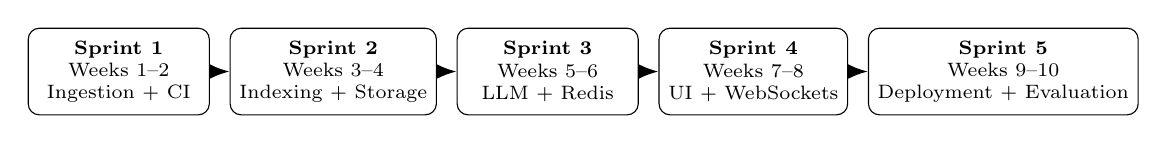
\begin{tikzpicture}[
    box/.style={
        rectangle,
        rounded corners,
        draw,
        align=center,
        minimum width=2.3cm,
        minimum height=1.1cm,
        font=\scriptsize
    },
    arrow/.style={
        -{Latex[length=2.5mm]},
        thick
    }
]

\node[box] (s1)
{\textbf{Sprint 1}\\Weeks 1--2\\
Ingestion + CI};

\node[box, right=0.25cm of s1] (s2)
{\textbf{Sprint 2}\\Weeks 3--4\\
Indexing + Storage};

\node[box, right=0.25cm of s2] (s3)
{\textbf{Sprint 3}\\Weeks 5--6\\
LLM + Redis};

\node[box, right=0.25cm of s3] (s4)
{\textbf{Sprint 4}\\Weeks 7--8\\
UI + WebSockets};

\node[box, right=0.25cm of s4] (s5)
{\textbf{Sprint 5}\\Weeks 9--10\\
Deployment + Evaluation};

\draw[arrow] (s1) -- (s2);
\draw[arrow] (s2) -- (s3);
\draw[arrow] (s3) -- (s4);
\draw[arrow] (s4) -- (s5);

\end{tikzpicture}%
}

\caption{10-Week Agile Development Roadmap}
\label{fig:roadmap}

\end{figure}

% -----------------------------------------------------
% 8. Engine availability heuristic
% -----------------------------------------------------

\section{Engine availability heuristic}

A mature set of ``engines'' (tooling/services) is available to implement this as a web-based project:

\begin{itemize}[leftmargin=0.7cm]

\item \textbf{Web framework:} FastAPI (Python) for asynchronous REST log ingestion and WebSocket streaming.

\item \textbf{Managed relational / search database:} PostgreSQL for structured incident storage and Elasticsearch for high-performance log querying and indexing.

\item \textbf{Caching \& rate-limiting engine:} Redis for in-memory signature caching, response reuse, and WebSocket session management.

\item \textbf{AI inference engine:} Groq API (Llama 3 inference) or local Ollama instances for low-latency stack trace translation and Root Cause Analysis (RCA).

\item \textbf{Test framework:} \texttt{pytest} and \texttt{httpx} for unit, schema validation, and API integration testing.

\item \textbf{CI runner and staging deployment target:} GitHub Actions for automated linting/tests and Render / Vercel containerized staging environments.

\end{itemize}

We will use these mature components to focus on workflow design, caching logic, and measurement rather than inventing new infrastructure.

% -----------------------------------------------------
% 9. Project scope and deliverables
% -----------------------------------------------------

\section{Project scope and deliverables}

\subsection{Initial deliverable}

\begin{itemize}[leftmargin=0.7cm]

\item Ingestion REST endpoint to receive structured JSON and raw text log streams.

\item Database schema setup (PostgreSQL) with automated timestamp logging for MTTD measurement.

\item Synthetic mock log generator script simulating microservice errors (database connection drops, payment timeouts).

\item CI: build + backend unit tests + linting via GitHub Actions.

\item CD to staging environment via a single containerized pipeline job.

\end{itemize}

\subsection{Subsequent deliverables}

\begin{itemize}[leftmargin=0.7cm]

\item Automated LLM-driven error parsing and plain-language RCA generation.

\item Redis caching layer to suppress duplicate AI API calls during high-frequency error spikes.

\item Real-time React dashboard with live WebSocket log streaming and error velocity charts.

\item Incident triage workflow (\texttt{Open} $\rightarrow$ \texttt{Investigating} $\rightarrow$ \texttt{Resolved}) with webhook notifications to Discord/Slack.

\item Benchmark evaluation suite measuring sustained log throughput and cache hit rate under load.

\end{itemize}

% -----------------------------------------------------
% Figure 5: Incident Triage Workflow
% -----------------------------------------------------

\begin{figure}[htbp]
\centering

\resizebox{\textwidth}{!}{%
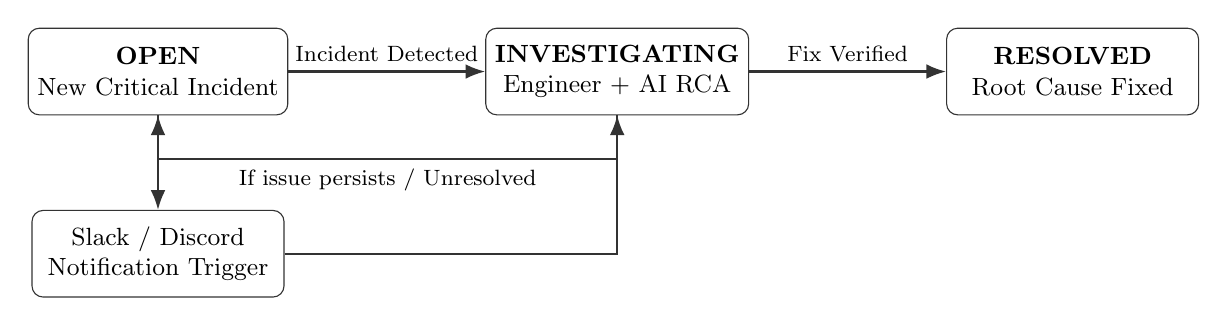
\begin{tikzpicture}[
    node distance=1.4cm and 2.5cm,
    state/.style={
        rectangle,
        rounded corners=4pt,
        draw=black!80,
        fill=white,
        align=center,
        minimum width=3.2cm,
        minimum height=1.1cm,
        font=\small
    },
    arrow/.style={
        -{Latex[length=2.5mm]},
        thick,
        draw=black!80
    }
]

% Main State Progression
\node[state] (open) {\textbf{OPEN}\\New Critical Incident};
\node[state, right=of open] (investigating) {\textbf{INVESTIGATING}\\Engineer + AI RCA};
\node[state, right=of investigating] (resolved) {\textbf{RESOLVED}\\Root Cause Fixed};

% Supplementary Alert Node
\node[state, below=1.2cm of open] (alert) {Slack / Discord\\Notification Trigger};

% Forward Transitions
\draw[arrow] (open) -- node[above, font=\footnotesize] {Incident Detected} (investigating);
\draw[arrow] (investigating) -- node[above, font=\footnotesize] {Fix Verified} (resolved);

% Alert Transitions
\draw[arrow] (open) -- (alert);
\draw[arrow] (alert) -| (investigating);

% Feedback Loop
\draw[arrow] (investigating.south) -- ++(0,-0.55) -| node[pos=0.25, below, font=\footnotesize] {If issue persists / Unresolved} (open.south);

\end{tikzpicture}%
}

\caption{Incident Triage and Resolution Workflow}
\label{fig:incident-workflow}

\end{figure}

% -----------------------------------------------------
% 10. Risks and Mitigations
% -----------------------------------------------------

\section{Risks and Mitigations}

\begin{itemize}[leftmargin=0.7cm]

\item \textbf{API Rate Limits / Cost Spikes:} Mitigate by using local LLMs (Ollama) or free-tier Groq APIs backed by aggressive Redis caching.

\item \textbf{Log Ingestion Backpressure:} Mitigate by using asynchronous background tasks and queueing log streams to avoid blocking main threads.

\item \textbf{Data Privacy / Sensitive Information:} Implement regex maskers on the ingestion pipeline to strip passwords, API keys, and PII prior to storage or LLM processing.

\end{itemize}

% -----------------------------------------------------
% 11. Summary
% -----------------------------------------------------

\section{Summary}

This proposal details an actionable, engineering-focused software project designed for a 10-week Agile development cycle. By prioritizing rapid time-to-value, automated CI/CD releases, clear metrics (MTTD), and practical full-stack AI integration, the project directly solves real-world DevOps triage delays while delivering a high-impact, production-grade resume piece.

% -----------------------------------------------------
% END DOCUMENT
% -----------------------------------------------------

\end{document}
